\documentclass{article}

\usepackage{fontspec}
\usepackage[no-sscript,no-logos]{xltxtra}
\usepackage{fancyhdr,setspace,tabu,refstyle,varioref,pgfplots,graphicx}
\usepackage[small,compact]{titlesec}
\usepackage[autostyle]{csquotes}
\usepackage[strict,notes,backend=biber]{biblatex-chicago}
\usepackage[multiple,marginal,bottom]{footmisc}

\addbibresource{citations.bib}
\setromanfont[Mapping=tex-text]{Linux Libertine O}
\setlength{\headheight}{15.2pt}

\setcounter{secnumdepth}{0}

\pagestyle{fancy}
\fancyhf{}
\renewcommand{\headrulewidth}{0pt}
\fancyhead[L]{Framing Political Interaction as Conversation}
\fancyhead[R]{\nouppercase{\leftmark}}
\fancyfoot[C]{–\ \thepage\ –}

\setstretch{2}
\begin{document}
\title{Framing Political Interaction as Conversation}
\author{Sam Stuewe\\ Professor David Blaney 
   \\ Professor Andrew Latham}
\maketitle
\thispagestyle{empty}
\newpage
\tableofcontents
\thispagestyle{empty}
\newpage
\setcounter{page}{1}
\section{Introduction}
For years, political thinkers have attempted to use metaphors to simply explain political interaction. 
Perhaps the simplest metaphor used for this purpose hails from the Realist tradition: all actors involved in an interaction are solid billiards balls whose internal setups are of no concern to the analysts and whose interactions with other actors are reduced to hitting one another which may be helpful or hindering.\footcite{mearsheimer01} 
However, like many of the metaphors that have followed, this framework fails to grasp the complexity of the situation at hand. 
It can be argued that the major benefit from these models is that, despite the loss of some detail, they make a complex situation easy to understand. 
Unfortunately, as the saying goes, ``the devil is in the details,'' and dismissing complexity in favor of simplicity only leads to the creation of a model without application. 
More ``leftist'' political theories, such as social constructivism, have offered less overly-simplified metaphors which allow for much more complex understandings, but often lead to such high-level abstraction that it becomes difficult for lay persons (or even modern politicians) to apply them in a given interaction.

In recent years, political interaction has fallen into categories that many of these models have difficulty understanding. 
Most obvious in this category (widely, and problematically, referred to as ``protest politics'') took the shape of the Occupy movements in concert with the ``Arab Spring.'' 
Realism largely disregards these movements as being outside the view of important actors despite their mass impact; social constructivism on the other hand is very capable of discussing the structures which have led to these protests and the systems in which they operate ignoring that the founding principle of these protests was to advocate for an escape and reformation of the structures themselves not of their subordinate policies. 
Thus, I intend to propose a new framework, one that has been in use for a long while but has not yet been formalized. 
Its goal is to provide a level of depth and complexity such that a wide variety of interactions may be fruitfully described and analyzed while remaining simple and accessible enough that people who do not identify as political theorists may still find it useful. 
To be clear, unlike \textit{realpolitik}, this is a framework meant to facilitate understanding, not a model meant to allow prediction. 
Through this framework, I will argue that the Occupy protests were not a fundamentally new type of political interaction, but rather a new manifestation of an older concept. 
Further, I will argue that Occupy is a scalable phenomenon and, therefore, may be applicable to international contexts. 
To make this argument, I must first make my foundational claims clear. 
So I will begin by discussing the origins of this framework and how it has evolved. 
Then, having established its background, I will elaborate on the framework itself and make clear its components. 
Using the elaboration of its components, I will seek to create a functional typology of political interactions. 
And finally, using this framework and typology, I will analyze Occupy on several cases of scale to establish its scalability.

\section{Intellectual Origins}
\seclabel{origins}
[Introduction to Lit Review]
\subsection{Location}
The notion of an arena in which political interactions take place is not a new concept and the exact meaning of the term has not always been well-defined. 
For some political scientists, it defines, at its most basic level, a sense of scope---e.g., the ``international arena.'' 
However, for Henry Mintzberg, for example, an arena is less a definition of scope as much as it is a description of duration. 
In his text ``The Organization as Political Arena,"\footcite{mintzberg85} Mintzberg refers to arenas as being particular situations of political interaction characterized by a form of organized conflict. 
He posits a typology of political arenas for which the defining characteristic which differentiates the cases are how the organization of the arena is constituted (primarily in terms of the intensity of the conflict, how well contained the conflict remains and for how long the conflict lasts).\footcite[141]{mintzberg85} 
Mintzberg's typology is founded upon the notion that all organizations are oriented around conflict and that because of the trends of conflict in politics, there are only four basic types of arena.\footcite[These four types are ``Confrontation,'' ``Shaky alliance,'' ``Politicized organization,'' and ``Complete Political Arena.'']{mintzberg85}
The most useful component of this model is its simplicity. 
As with other seemingly predictive models, given various input factors (of which there are not many possibilities), probable outcomes may be predicted with confidence. 
But the notion of a political arena as being only valuable with reference to conflict implicitly dismisses cooperative political interaction;\footcite[152]{mintzberg85} and, even more distressing, his model assumes a vacuum-sealed environment. 
That is, there is little to no context shaping the arena before the conflict becomes apparent. 
No political interaction is without context and without giving some analysis focused on the context which gave rise to, or influenced, the interactions themselves, a great deal of useful information (which will assuredly affect outcomes) is lost.
A more helpful theory of location would establish the relationship between the different types of arenas as culminations of various contextual factors which guide the evolution of the arena itself and which influence the eventual participants and actions which take place in it.

Giving an extra dimension to the contextuality of interactions, Anthony Giddens's theory of ``structuration''\footcite{giddens86} offers a model for understanding the existence of institutionalization.
In particular, Giddens traces the unintended consequences of a given action to becoming conditions which influence future actions.
However, because of their having arisen unintentionally, they are overlooked or unacknowledged in the calculus of future actions.\footcite[5]{giddens86}
The repetition of this cycle leads to the embedding of these unacknowledged action-influencing conditions, or institutionalization.
This notion of institutionalization brought about through overlooked conditions is at the heart of the concept of normalization---an integral part of understanding how institutions become internalized.
Yet, though Giddens speaks, at great length, about the separations between intended and unintended consequences, he glosses over the possibility for \emph{intended} consequences to play into the same framework of overlooked conditions which internalize norms.
That is, it is entirely conceivable that a political actor could influence future actions through intentional decisions which would still go overlooked by other actors. 
More important than these notions of internalization, however, is Giddens's argument surrounding the ``duality of structure.''\footcite[16]{giddens86}
Through this mechanism, Giddens argues that not only do institutions shape future actions, but each action reproduces the institution (which may be reinforcing or modifying).\footcite[19]{giddens86}
Thus, the institutions which constrain action are created and recreated by action itself.

Drawing on Mintzberg and Giddens, the notion of a political arena---of a location in which political discussion can take place---has several basic characteristics.
It is organized and created by actors who shape its character.
The organization of the location influences (sometimes obviously, and other times subversively) future actions taken.
Finally, the organization and the action are mutually generative and reinforcing---each produces and reproduces the other.
With this basic concept of a location in mind, it is necessary to step forward to see what theorists say about the participants in interaction.

\subsection{Participants}
While the location and context of any political interaction holds great importance, those who participate in the interaction itself are, perhaps, the primary subjects of interest. 
In the intro to his work, \emph{A Semisovereign People}, E. E. Schattschneider, like Mintzberg, frames political interaction as conflict and confrontation as it relates to participants.\footcite{schattschneider75} 
In particular, his model focuses on an argument taking place in a hotel lobby.\footcite[1--5. Ironically, despite mentioning the location of the conflict, Schattschneider fails to discuss how the location may have affected the interaction.]{schattschneider75} 
In this argument, as in Schattschneider's framework as a whole, the focus should be placed on the ``audience,'' not the ``speakers.'' 
He pays special attention to the size of the audience as this is what, he claims will play the decisive role in determining the outcome of the conflict: 
\blockquote{\setstretch{1}The logical consequence of the foregoing analysis of conflict is that the balance of forces in any conflict is not a fixed equation until \emph{everyone} is involved. If one tenth of \oldstylenums{1} percent of the public is involved in conflict, the latent force of the audience is \oldstylenums{999} times as great as the active force, and the outcome of the conflict depends overwhelmingly on what the \oldstylenums{99.9} percent do. Characteristically, the potentially involved are more numerous than those actually involved. This analysis has a bearing on the relations between the ``interested'' and the ``uninterested'' segments of the community and sheds light on interest theories of politics. It is hazardous to assume that the spectators are uninterested because a free society maximizes the contagion of conflict; it invites intervention and gives a high priority to the participation of the public in conflict.\footcite[5]{schattschneider75}}\setstretch{2}
Here, Schattschneider offers a great number of helpful concepts. 
For example, he offers us the concept of interest as it relates to participants (though he makes this distinction as only being important with reference to audience members and not vocal participants). 
However, perhaps most important, he makes obvious that the dynamics of an interaction are ever-changing. 
Unfortunately, Schattschneider's model focuses almost entirely on the participants (and, even then, very heavily on the audience and not the vocal participants). 
Furthermore, not all political interaction can be accurately characterized as conflict. 
Therefore, his model is simply not applicable to some cases, and despite the utility of many of his concepts, his model overall is too focused on only one aspect of any given case.

Combining some of Schattschneider's insights with the basic concept of a location, the concept of participant dynamics begins to take shape.
Though Schattschneider places a (perhaps undue) large emphasis on the non-vocal participants, it is clear that the relationships between participants in the conversation matters a great deal, and that the construction of the location might have serious implications as to the status of those relationships.

Susan Bickford, similar to Schattschneider and Mintzberg, still assumes a level of conflict evident in political interaction but focuses on a different part of participants and their relation to the conversation as a whole.
In particular, her text \emph{The Dissonance of Democracy}\footcite{bickford96} focuses on listening and how much it affects conversations disproportionate to how much it has been addressed in academic literature. 
Referencing Plato's \emph{Republic}, Bickford argues that communicative interaction is founded on the understanding that those making arguments will have an audience willing to listen.\footcite[3]{bickford96}
This realization is extremely useful as it offers a basic cast of participants and their roles in a conversation.
Fundamentally speaking, arguments rely on having multiple participants who play various roles (moving between orator and interpreter).
Beyond this realization, it highlights an extremely powerful action for audience members to take: not listening.\footcite[3]{bickford96}
Bickford makes note that pre-cursory agreements determine rules of interaction such that various means of decision-making become normalized.\footcite[3--5. Simply put, these pre-cursory agreements can be understood as ``constitutions''---both formal and informal institutions which govern interaction.]{bickford96}
These agreements are often made to allow for preferring majority rule or another consensus-based mechanism in the place of the use of force.
Bickford's argument is particularly useful because it does not empower ``listening'' to the disenfranchisement of ''speech,'' but rather equalizes the playing field for both claiming that politics itself is ``about the dynamic between the two.''\footcite[4]{bickford96}
Furthermore, it does not assume conflict is the only character of interaction.
She asserts a complex understanding of relationships (through connections and divisions) which influence actions through affects on the dynamics of any given conversation.\footcite[9--11]{bickford96}

Now, with the addition of Bickford's notion of speech and listening as being complimentary and the roles associated with both activities, the dynamics between participants are far more clear.
Coupled with the notion of presence as it relates to position in a given location (particularly that a given position may tip the scales of influence in favor of the participant which holds that position), the stage is set for the possibility of discussions taking place between these participants to be weighted in favor of particular parties, and for those discussions to be heavily shaped by the context in which they arose.
Thus, I turn to the content of the conversations itself and how it has evolved in academic literature.

\subsection{Content}
With his focus set on the final aspect of political interaction, Jeffrey Banks's \emph{Signaling Games in Political Science} concentrates on information transition, or ``signaling.''\footcite{banks91} 
Banks's analysis focuses on signaling games (particularly incomplete information signal games\footnote{He argues that models which allow for complete information have very little predictive and intellectual merit due to serious limitations on the applicability of the model in real situations}) and how political interaction can be cast in the light of these games. 
Despite his focus on game theory (which emphasizes predictiveness), Banks still offers a prototypical model of politics as conversation. 
In his case analysis, he cast the model's ``players'' as speakers and the signals sent which may influence other players' actions as ``speeches.''\footcite[37]{banks91} 
For Banks, there are two well-defined players, the ``sender'' and ``receiver,'' and there is little acknowledgment of any response.\footcite[4]{banks91} 
That is, where Banks imagines, at most, a one-directional message being sent, a more realistic metaphor would describe messages being sent back and forth between multiple participants which often mutually influence one another. 
Banks's model greatly limits the scope of its application through its implicit definitions. 
For example, the only signals Banks concerns himself with are those which influence others by limiting the receiver's set of choices through a mechanism he refers to as ``agenda control.''\footcite[3]{banks91} 
Not only does this cut out all cases of interaction in which the effects are undetermined, but it undermines the understanding of interactions as being more than just unidirectional. 
Furthermore, Banks's notion of influence is a very traditional definition of power (where an actor limits another actor's ability to do something or expressly forces them to do something they otherwise would not) for the sake of the model's application for prediction to the detriment of its complexity. 

However, despite all the limitations Banks places on his model, it remains surprisingly versatile. 
In his case analysis, he applies his model to literal cases (candidates making speeches to audiences) but makes it generalizable through a metaphor by which analysts may understand much higher-level games through the same terms. 
This is what makes Banks's model so appealing; despite all its limitations, it is scalable.
That is to say, Banks clearly creates many (perhaps) artificial constraints on his model in the name of predictiveness, but the model itself is helpful for understanding situations which he would never have considered.
In particular, his notions and the language he uses surrounding the concept of signaling are useful for describing any action made at any scale of interaction (be it between two individuals or between two nation-states).

Adding Banks's insights into the content of a conversation to the more complex picture of participant dynamics that Bickford offers creates a much more helpful understanding of how conversation is conducted.
Conversation takes place when messages are sent between participants who then interpret them and respond.
Each message is influenced not just by the sender(s) and receiver(s), but also by the environment which has brought the participants together and established the dynamics and context for the conversation in the first place.
In the next section, I will offer a metaphor---founded in the terms which have been used throughout the paper up to this point---to help clarify the relationship between each aspect of conversation.

\section{Conversation as a Metaphor}
In their seminal work on metaphor, George Lakoff and Mark Johnson argue that metaphors are deeply pervasive and that humans fundamentally rely upon metaphor.\footcite[3--6]{lakoffjohnson80}
Throughout their text, \emph{Metaphors We Live By}, they seek to show the use of metaphor as being applicable to a great many aspects of human life.
With their framework of metaphor in mind, I will attempt to construct a unified framework for political interaction grounded primarily in a ``structural'' metaphor of conversation.\footcite[14]{lakoffjohnson80} 
The inherent advantage of this type framework is that it draws on a construct that would be simple for any academic or lay reader to access and analyze.
Thus, I will attempt to create a comprehensive framework for political interaction using this metaphor; however, even if it should not, any intellectual extension of the framework should be discoverable through little more than logical exploration.

This metaphor of conversation has three general components which were discussed throughout section 2.
These are the \emph{location}, the \emph{participants} and the \emph{content}.
Without discussing all three components, a vital piece of information---which may be critical to useful analysis or generalization---is lost.
Each author discussed before has offered a number of valuable concepts which, when developed further and are synthesized, offer a far more realistic and revealing picture of political interaction.
What follows is the initial construct of a metaphor of conversation for political interaction.

\subsection{Imagine a Room}
In this room, there are an indeterminate number of walls, doors and windows.
Some of the walls have been added in such a way that they form small enclaves within the larger room itself.
Both the doors and windows vary between open and closed states; and on occasion, some are removed entirely or are newly installed.
The room itself was built a long time ago (though there was never an exact moment when construction was started).\footnote{Though it is outside the scope of this work to establish, the concept of a well-defined line between a ``state of nature'' and modern society has been soundly questioned. To reflect this, assume that this room has been evolving through construction and maintenance without a clearly defined beginning.}
Due to the construction and previous alterations, this room's acoustics and floor are uneven which amplify some voices while effectively muting others. 
Finally, despite this room's having changed (significantly) over time, alterations made to the room take a great deal of time to complete, and often happen as individual projects to change very small characteristics.

This room, however, is far from empty. There are many people inside at any given moment whose focus varies greatly.
Some of these people are focused on discussions taking place within the room itself, while others are more concerned with those going on outside.
There are also, of course, some people outside the room looking in through a window or open door, and many people will either move from the inside out or vice versa quite often.
Regardless of where people are in the room, they serve two roles (often simultaneously): that of the speaker and that of the listener.\footcite[4]{bickford96}
Like any other room, movement inside is fairly unencumbered, but each person is given an assigned seat, which rarely changes, where they are expected to sit for most discussions.\footnote{Though they are \emph{expected} to sit in their assigned position for the most part, they are not (typically) physically required to do so.}

Understanding that the characteristics of the room and the people inside it have a great deal of influence on the topic, imagine a discussion taking place in this room.
Its organization is governed by the physical limitations of the room and by agreements made between participants.\footnote{Which are created through discussions held before-hand (e.g., the seating arrangement)}
Though the topic is often determined by those inside the room taking part in the discussion, it may concern those outside as well.
The topic of discussion may morph and change as various statements are made.
Various people in the room will understand the topic in a different light, which will color their speaking about and listening to discussion concerning it.
Statements and questions made will often be of a certain tone which reflects the speakers' opinions surrounding the topic.
And, the tone of various statements can greatly affect the responses which they may garner.
Each discussion in this room may seem as though it has a well-defined beginning and end, but such is not the case.
Discussions often (if not, always) flow from one into another even if they do not fundamentally change either the room or its participants.

\subsection{Grounding the Metaphor}
[Finish cross-references to authors in lit review]

The locational aspect of this metaphorical room serves to represent the systems of rules, norms and physical limitations which govern modern political interaction.
These norms and systems were ``created''\footnote{A problematic term because it validates the view that a well-defined moment of consensus which brought humankind out of a state of nature and into society---a fiction.} long ago and have been evolving ever since.
The walls, windows and doors highlight the separations---which are often artificial in nature---between those involved in the conversation and those who are not.
Furthermore, the notion of enclaves establishes the possibility of separations between participants who \emph{are} all involved in the conversation.
The openness of the doors and windows are meant to make clear the traversability of these artificial boundaries and allow for a basic mechanism for joining and leaving a given discussion.
But the interior of the walls describe a separate characteristic.
The acoustics of a room (i.e., how sound reverberates through a space) are heavily determined by the arrangement, construction and decoration of the walls.
With little modification to the walls alone, a room can be made to amplify or mute sound coming from a particular point.
These acoustics serve to demonstrate how an institution (physical or abstract) might benefit the voice of some over others solely because of their relative position.
In deeper detail still, the varying height of the floor provides, perhaps, a more clear obvious example of a lack of equality in constructs of conversation.
The final metaphorical detail I offer about the room itself is meant to establish a sense of longevity.
Where the metaphor explicitly allows for participation to change drastically, and discussion contents are nothing but ephemeral, the construction itself (though it can be modified) resists drastic change.

In contrast to the locational aspect, the participational aspect of the metaphor represents the focus, relationships and possible actions which describe the participants in a given discussion.
The focus of the participants speaks to their attentiveness to particular conversations or traits of those conversations---for example, are participants actively engaged in a conversation, or are they more interested in one taking place further away (or even one taking place outside the room itself)?
Despite how attentive a participant may be, however, they will still be part of a conversation by means of both their active presence and passive lack of absence.\footcite{bickford96,giddens86}
The entering and exiting of the room is an extension of the dichotomy of presence and absence; namely, it offers a simple mechanism by which participants can remove their influence (whatever influence they may have) from the conversation,\footnote{Perhaps ironically, or maybe just fascinatingly, this willful departure from asserting direct influence is itself a statement made in the conversation which may carry great power.} or by which they may attempt to assert influence by entering the room having been outside.
The motion within the room and the seating arrangement are meant to evoke an understanding that participants inside the room \emph{do} have some autonomy.
As various conversations may be taking place at any given moment in the room, participants may wander so that they may hear better.
Of course, this freedom of movement is largely cosmetic; to change one's position in the room permanently is much more difficult.

Finally, the content-oriented aspect represents the organization, topic, tone and duration of the conversation itself.
All pieces of this aspect are determined almost entirely by the location and participation.
However, the influence from the location and participation is comprehensive, so the participants outside the room may have a great deal of influence on the topic.\footnote{Perhaps, on occasion, more so than those inside? See: note 31}
Unlike the relative stability of the room itself and even more obvious than the fluidity of change in the participants, the nature of the conversation can change very swiftly.
Each singular statement made by a participant may be enough to shift the topic, and, to complicate the matter, the different identities of the participants will influence how they interpret the topic.
As intertwined as the rest, the tone of the conversation as a whole derives from the tone with which each participant makes a statement.
Thus, should participants speak with a tone of hostility, the conversation may begin to take on that character as a whole.
Finally, the notion that conversations are never well-defined is meant to reinforce the understanding that the process of a conversation does not end: each statement leads to further development which leads to more statements.

\section{Statements in Conversation}
Given this more complex (but still general) understanding of how conversations are created and how they unfold, I would like to turn the analysis of conversation in the direction of what type of statements can be, and are, made during a discussion.\footnote{I need to make clear at some point earlier that a discussion will be defined (problematically, but usefully) as an instance of a conversation characterized by a particular topic (or set of topics)}
Before I discuss the categorization and subsequent typology associated with statements, it is important to note that the term ``statement'' may be metaphorical or literal.\footnote{[Might remove this in favor of more clearly explaining the application of this framework in the intro/elsewhere]}
Each statement might be something \emph{literally said} by a person in the sense that Bickford and Mintzberg discuss, or could be as abstract as the speeches which concern Banks.\footnote{[Add citations]}
However, the language and rationale for understanding a conversation in either the metaphorical or literal sense remains the same.

Thus, I turn towards a typology of statements.
Each statement in a discussion may be categorized with reference to affecting the scope of one of the three aspects of a conversation.
A statement can either make more wide, cosmetically change or make more narrow the location, the participation and the content of a given conversation.\footnote{Might also be worth mentioning interruptions; statements made which cut off others before they finish}
The following table illustrates fairly broad categories through which widening, cosmetic change and narrowing may take place.
The horizontal axis describes which aspect is being affected by the statement whereas the vertical axis describes how that aspect is being affected.
For example, ``construction'' refers to the category of statements which \emph{widen} the \emph{location}; and, conversely, ``specification'' refers to the category of statements which \emph{narrow} the \emph{content}.
In the sections which follow the table, I will elaborate on how each type of statement can take shape and the effects it can have on the dynamics of a conversation.

\begin{tabu} [c] {c|c|c|c|}
   \multicolumn{1}{c}{} & \multicolumn{1}{c}{Location} & \multicolumn{1}{c}{Participants} & \multicolumn{1}{c}{Content} \\\cline{2-4}
   Widening & Construction & Inclusion & Generalization \\\cline{2-4}
   Cosmetic & Maintenance & Rearranging & Rephrasing \\\cline{2-4}
   Narrowing & Demolition & Exclusion & Specification \\\cline{2-4}
\end{tabu}

\subsection{Location}
As mentioned briefly in the metaphor elaborated in the section above, modifications made to a location take a fair amount of time compared to those relating to the other aspects.
Typically, these statements are made because participants believe each addition allows for more equity.\footnote{That is, not what is truly equal, but rather, what they consider to be \emph{fair}.}
These modifications can take the shape of construction, maintenance and demolition.
Construction, logically, involves the addition of a new installation to the room.
New additions can be anything from a new wall, window, doorway or even a small enclave or adjoining room.
Because of the amount of work required (along with the implications of the new separations, or entrances), these tend to be some of the most difficult statements to support.
Perhaps one of the best examples of construction in the sphere of international relations can be found by looking to the United Nations Security Council.\footnote{Concept is strong; need a citation to back it up.}
The \textsc{unsc} is given the power to establish subsidiary bodies as needed under the \textsc{un} Charter.
Over the years, a great many new subsidiaries have been created, primarily in the form of committees.
Each of these committees can be viewed as enclaves inside the room of the \textsc{unsc}; each may have several (seemingly) independent discussions taking place within at any given moment, but all of them are influenced and shaped by the larger context which gave rise to them.
In turn, each committee influences policy and rhetoric present in the \textsc{unsc} overall.

Unlike construction, maintenance focuses not on making drastic changes through creating new additions, but rather on reforming or revising those installations which have already been created.
Maintenance often takes the form of modifying the various heights of the floor or changing the acoustics of the room's walls through soundboards.
It is not uncommon for these statements of maintenance to reverse or reinforce previous pieces of maintenance.
These statements also have a strong chance of influencing indoor dynamics, but their effects do not appreciably increase or decrease the size of the room itself.
Again, one of the most obvious manifestations of maintenance lies in the history of the \textsc{un}---the formation of the United nations Human Rights Council.
The \textsc{unhrc} was established to replace a heavily criticized organization, the United Nations Human Rights Commission.
The goals of both were largely the same, but the structure of varied greatly.\footnote{Preliminary source: http://news.bbc.co.uk/2/hi/europe/4810538.stm}
This represented not a drastic addition of a new installation, but rather focused on reforming an older one.\footnote{This probably doesn't quite fit since it's an example of a replacement rather than a reformation. This may be a better example for when/if a discussion about replacements comes up in relation to demolition.}

Finally, demolition is the process of removing established installations.
Anything that can be added in construction can be removed in demolition (including the foundational structures of the room itself).
Though these statements can be controversial because they remove installations which have become part of the established order, they often involve much simpler proposals since they focus only on removal of an installation which may take much less work than the planning for an addition.\footnote{Only examples, to my knowledge, of \textsc{un} organizations that have been totally removed were the \textsc{chr} (mentioned above) and the \textsc{iro} which is a near identical example to that of the chr. Odds are one of those two examples will end up in this paragraph, and I will need to find a different example to use in the paragraph above.}

\subsection{Participants}
Much like statements which affect the makeup of the location of a conversation, those that affect the makeup of the participants can be categorized by their affect on its extent.
It is important to note that these statements are made much more often and are completed much more quickly than those which affect the location overall because the room, in general, facilitates movement.
These statements will either take the shape of inclusion, rearrangements or exclusion.
Statements of inclusion most typically come to bear in the form of invitations from, or demands made by, the indoor participants to entities currently outside.
However, they may involve invitations or acceptance of participants into smaller enclaves\footnote{Reference Enclaves} as well.
For example, one could look to the inclusion of nations as member states to the United Nations.\footnote{Or perhaps I should move the example of Occupy's ``\oldstylenums{99} percent'' here?}
Every new nation recognized as a member state is invited inside, so to speak.
With the inclusion of a new member, many organizations may be refactored to adjust to the new member, or the new member will adjust to the organizations in-place already.
However, the primary change is in the makeup and dynamic of the membership; each new member brings a new perspective and a new set of interests to the conversation.

Rearrangements, the more cosmetic change, most often affect the seating arrangement or speaking order of a given conversation.
These can drastically affect position in the room and can therefore make fundamental changes to the dynamics between participants in a given conversation.
However, because they do not affect who is welcome in a conversation and who is excluded, they will be far less controversial than inclusionary or exclusionary statements.\footnote{Must come up with a good example of this---\textsc{unsc} rotating membership?}

Finally, exclusionary statements are those which intentionally remove a participant from membership in the room itself or in a smaller enclave.
These statements may be made in order to exclude an individual, or they may be made by an individual to exclude themselves.\footnote{Hirschman and Fraser with exiting}
By again looking to the \textsc{unsc}, there is a simple example to be found.
Recently,\footnote{Preliminary source: http://www.nytimes.com/2013/10/19/world/middleeast/saudi-arabia-rejects-security-council-seat.html} Saudi Arabia was invited to take one of the rotating seats of the \textsc{unsc}, and declined.
In doing so, Saudi Arabia chose to exclude itself from the position offered.
This action may have been entirely rhetorical---i.e., an attempt to signal a lack of need for the \textsc{unsc}---but Saudi Arabia's Foreign Ministry released a statement noting that it declined because the \textsc{unsc} has proven to be ineffective and that it would gladly join the conversation were the body to prove itself useful.\footnote{preliminary ibid}

\subsection{Content}
Even more than participational statements, content-oriented statements are much more quickly made than those which concern the location.
Each single discussion can involve a great deal of these statements, and each statement has wide ranging immediate effects on the future of a discussion's content.
These statements most often take the forms of generalization, rephrasing and specification.
Generalizations are made to widen the content of the conversation by allowing for a greater variety of allowed statements.
That is, often through manipulation of terms or the topic itself, generalizations offer an avenue for more areas of discussion to be a part of the conversation.
Arguably, the best modern example of topic expansion arose with the Occupy movement.
In order to help bring about public discussion of issues that concerned many people of very different backgrounds, the issues important to each person were framed as being important to everyone.
That is, the topic of discussion was open-ended; anyone who wished to air a grievance was welcome to do so.\footnote{[citation needed]}

However, many times a statement is not well-received not because its scope is too wide or too narrow, but rather just because of how it was phrased.
As a result, cosmetic change arises in the form of simple rephrasing.
Rephrasing a statement can be as simple as using different terminology, but the motions of doing so may make the statement itself much more acceptable by other participants.\footnote{Think of a good example}

Finally, content-oriented statements may be made to narrow the topic through specifications.
Specifications, like generalizations, may be made through the terms of the conversation or more powerfully through the topic itself.
Making these statements can make future statements more efficient by focusing them on more specific goals; however, doing so will necessitate that other goals be left unattended.\footnote{Occupy's narrowing focus on wealth inequality as a good example?}

%\subsection{Outcomes}
%Unlike their counterpart category which seeks to end discussion, inquisitive statements are inherently hoping for a response.
%As a result, the forms they take are less subtle in nature.
%The two most basic categories into which inquisitive statements fall are assertions and questions.
%However, the separation between the two is more a matter of phrasing than it is one of inherent difference.
%Both manifestations are examples of statements made in a process meant to help the participants seek further understanding.
%The phrasing of the two determines the inherently defined agency given to the listener.
%A question includes a built-in agency for the listener to become a speaker and respond to what was asked.
%In contrast, an assertion makes no such offer to the listener, and should listeners wish to then take on the role of speakers and respond, they must find their own motivation and opportunity to do so.

%Despite being less common than inquisitive statements, rhetorical statements have vast implications.\footnote{[citation needed] or rewording to be less assertive}
%A rhetorical statement will be one made in the hopes that no response will follow where an inquisitive statement will be one made in the hopes that a response \emph{needs} to follow.
%Given the intended outcome of these two possibilities, the role each plays is fairly clear.
%Rhetorical statements are meant to end a discussion where inquisitive statements are meant to stimulate conversation.\footnote{Note: inquisitive statements are not necessarily intent on stimulating the specific discussion. They may very well be aimed at moving onto a different subject; but they hope to continue conversation.}
%A rhetorical statement can take two basic shapes.
%The first, an innocuous comment\footnote{Miniature statement?} which may add little to the conversation or a concluding statement to a conversation which attempts to settle an issue such that no response is necessary.
%The second, and far more contentious, radical silence.
%If a conversation, by definition, requires that there are multiple participants sending messages back and forth, then the possibility for a participant to choose not to part-take in the conversation can cause serious troubles for interaction.
%Bickford offers a prototype of this notion of ``not listening,''\footcite[pg]{bickford96} but radical silence can extend far beyond choosing to not listen.
%It can, at the most radical edge, culminate in the choice to exit the conversation entirely.\footcite{hirschman70}\footnote{Fraser, exiting and exterior rooms}
%Fascinatingly, doing so is one of the most likely actions to arouse responses, but such an action can, by definition, bring a conversation to its end almost instantly.

%[transition]

%\subsection{Scope}
%Each type of statement has a varying degree of effect.
%Those statements which focus on creating change in the conversation will have a greater scope because they are more likely to concern more participants.
%Following logically, statements made with the intention of eventually bringing about change at more fundamental levels of the conversation will have a wider scope than those which do not.
%For example, a statement made with the intention of changing the topic of discussion itself will not have a wide scope unless the discussion being switched to, or from, has implications for the participants.
%On the other hand, a statement made with the intention of fundamentally changing the organization or structure of the location will have a vast scope because it directly concerns every participant involved in the conversation.

%[Deeper elaboration on which statements have a wider or narrower scope]

%[Transition]

%The content of the conversation changes often and is heavily (if not, entirely) influenced by the location and the participants.
%It can be thought of as having several basic characteristics: topic and tone.
%Each conversation must intuitively have a topic.
%This topic can be anything the participants might propose and the room allows.
%The realm of allowable topics may include anything from new alterations for the room to the dismissal or welcoming of a new person to the room (or even a particular discussion).
%Perhaps this is because the precursory agreements which participants agree to in order to join a conversation in the first place strongly discourage leaving.
%An Innocuous Rhetorical comment will have little effect on the conversation as a whole and will serve more as punctuation or a footnote for previous statements made.

Over the course of the next section, I will seek to analyze the Occupy movement on varying levels of effect in terms of the typology explicated above.
In particular, I will focus on several watershed moments of the movement, their lasting effects, and some examples of messages which never got the recognition that the more pervasive messages did.
Occupy must be recognized as a movement with an effect on, at least, three different levels of interaction: metropolitan, national and international.
In this section, I will offer a short history of Occupy itself and then delve into the intricacies of each level as a separate case.
Each case applied different strategies---and, as a result, different statements---which colored the effectiveness of each message and, when viewed in terms of the framework and typology laid out above, make clear the lasting effects.

%[MOAR TRANSITION]

\section{A brief history of Occupy}
In light of the Arab Spring protests and various occupations in Greece and Spain, Adbusters (an online blog with a history of social justice motivations) began calling for similar movements to happen in the United States.\footnote{https://www.adbusters.org/blogs/adbusters-blog/occupywallstreet.html}
That is, Adbusters advocated for protests that highlight inequalities and other issues of civil interest that government bodies appear to have ignored.
On \oldstylenums{17 September 2011}, the occupation of Zuccotti Park began, and the Occupy movement in the United States was born under the banner of a Twitter hashtag (\#OccupyWallStreet).
Over the course of the next several months, similar occupations began in cities across the United States such as Washington, \textsc{d.c.}; Kansas City, \textsc{mo}; and Saint Paul, \textsc{mn}.\footnote{I know I cannot/should not cite Wikipedia; nor do I intend to. But, for now, see this list: https://en.wikipedia.org/wiki/List\_of\_Occupy\_movement\_protest\_locations\_in\_the\_United\_States}

Through the use of consensus-based General Assemblies, the various occupations each had their own focuses of issues they felt central to improving life for all people in the United States.\footnote{Good time to talk about the \oldstylenums{99} percent rhetoric}
Each General Assembly served as a semi-centralized forum for making decisions on behalf of the collective occupation.
The areas of decision-making ranged from stances on various issues to over-arching ideological issues.
And, for each issue area, a committee was created---using very similar mechanics---which would meet ahead of time to determine the most important topics to be proposed at the Assemblies.
For an example of the issue areas, one of the primary misconceptions held about Occupy was that it was a movement without express purpose.\footnote{Citation needed}
This perception most likely arises from Occupy's lack of advocacy for a particular policy.
Contrary to popular belief, this lack of clear policy advocacy was entirely intentional.
One of the earliest committees formed was one concerning policy advocacy.
However, the Assembly overall remained resolute that the real problems the movement should address could not be resolved through policy (and require systemic change).

Not long after the occupations began, several cities opted to evict the protesters from their locations (most notably the Wall Street eviction on 15 November).
Though slowed by the semi-forced transition away from physical occupation, the protest movement did not cease with the evictions.
Rather, the movement has shifted course significantly.
Now, rather than focusing on outright protests, Occupy has transformed significantly to lobby for social change through other means.

[Transition to Cases]

\section{Wall Street}
Occupy in the United States is most well-known for Occupy Wall Street (\textsc{ows}).
This is not only because it was the first in the series, but also because of how the movement spread through the public eye.
Information spread about Occupy often using one hashtag, \#OccupyWallStreet, even though it did not correctly highlight the separation between each site.
Even news media focused most heavily on the protests in Zuccotti Park.
This being the first, and largest of the protests, it is arguably the best location to use as an example of a local-level case.

\subsection{Initial Occupation}
%Perhaps one of the gravest mistakes of the public has been to label Occupy as a movement without plan or direction, but instead one of unbridled spontaneity.\footnote{Find any few news sources for this; there should be many}
%On the contrary, despite the appearance of spontaneous 
%With as much a focus on deliberative democratic involvement as the Occupy General Assemblies held, it is no accident that Occupy took income inequality as a primary issue.
The initial occupation of Wall Street serves as one of the most easily catagorizable statements made throughout the whole Occupy movement.
Upon the achievement of consensus that the current structure of society and government fails to address issues of civil interest, the decision is made to help construct a new space for discussion that might fill the void.
This piece of construction was focused at addressing, among other things, the inequality perceived in the realm of discourse.
Thus, the movement never sought to elect candidates to office---it was never a goal of Occupy to change politics from inside the current system.
Rather, \textsc{ows} created a space \emph{outside} normal politics meant to facilitate systemic change \emph{inside}.

Yet, Occupy is not solely a manifestation of construction.
After the occupation itself began, the rhetorical strategies employed were crafted to embody the messages of the change they hope to create.
That is, \textsc{ows} sought to practice what it preached by realizing some of the social changes it hoped to see nationally in its own governance.
Most obvious, from an analytic standpoint, would be the direct nature\footnote{It would be wrong to say that Occupy supported direct democratic involvement. Democracy is founded on the notion of majority-rule; Occupy was founded on the notion of consensus. Democracy is not ``democratic'' enough.} of the decision-making structure of the occupation itself, but that is likely not the most well-known example.
Perhaps the best-known example of this ``practice what you preach'' policy was the ``\oldstylenums{99} percent'' slogan.\footnote{This ¶ may be better in the National Section}
Occupy saw a great many people (the overwhelming majority, in fact) as having almost no voice in their government and with no capacity to change such a reality.
The use of the ``\oldstylenums{99 percent}'' slogan was meant to energize and mobilize the very population it refers to (i.e., everyone save those who allegedly already control politics\footnote{This is not meant to be so politically charged. I either need to rework this to be nicer, or find a quote}).

Beyond construction, the occupation's system of self-governance through General Assemblies served as a statement of inclusion---one meant to help incorporate the disenchanted and disenfranchised members of society into the discussion so that they might have increased agency.
By doing so, \textsc{ows} reaffirmed its concentration on mass political involvement, but even more, it began the groundwork to create new (and strengthen established) communities which continue to work for the betterment of society.

\subsection{Responses to Occupy}
In short order, ``wealth inequality'' had been identified as one of the primary causes for many of the problems identified.
However, Occupy remained intent on being a forum for the spread of information and awareness, not an actor advocating for policy change.
Perhaps due to frustration with the movement's lack of a clear policy goal, or maybe simply because of the inconvenience, Michael Bloomberg, Mayor of New York City, decided that the occupation must end.
Regardless of the motivations, the eviction was clearly a statement in itself.

At first glance, the eviction appeared as a statement of destruction---as seeking to remove the space that had been created for the new discourse.
Yet, it cannot be so simply classified.
One of the cited motivations for the evictions was a need to clean Zuccotti Park of hazardous materials and to keep the premises safe.
It is worth noting that Zuccotti Park is private property. 
This status has serious implications for the legality of the occupation, but oddly, it never became a decisive issue.
It does, however, lend serious legitimacy to the eviction.
One of the reasons the eviction did not take place sooner was because Zuccotti Park was private property---the government had no authority to remove any person from the premises unless illegal activity was suspected or at the request of the owner. 
This means that the eviction must have, at the very least, been approved by the owner---it may have even been requested.
After the cleaning had completed, the protesters were allowed to return to the park, though new regulations had been added stipulating that protesters may not lie down or sleep in the Park.
Given that the space was reopened for protesters to use (and that the eviction was almost certainly approved by the property owner),\footnote{Citation Needed} it may be best to characterize the evictions not as statements of destruction, but rather as statements of maintenance---made to keep the new space up to standard by constraining the movement through regulation.

On the other hand, the new restrictions implemented effectively destroyed any option for an extended physical occupation.
In that sense, the evictions were not maintenance so much as they were destruction mixed with exclusion.
By implementing restrictions that severely decreased the time that people can spend in protest, the number of people able to participate was also significantly lessened.\footnote{Citation Needed}
Though a large majority of Occupiers were found to be wealthy individuals,\footcite[10]{milkman13} a considerable number of them were homeless.
With no ability to physically occupy the Park for extended time, many could not stay in the area at all.\footnote{\textsc{Ows} was not the only site to have such issues; OccupyMN (later OccupyMpls, or \textsc{ompls}) faced many of the same issues.}

\subsection{Working Forward}
Most fascinatingly, though Occupy did not end with the evictions (and there \emph{are} still physical occupations and protests that continue to the time of writing this document), news organizations almost entirely ceased covering the movement.\footnote{Perhaps this was because it became more difficult to track when it became less centralized (but this seems unlikely as the internal media organization and resources are just as easy to reach today as they were in the midst of the occupations)}
Each site had different means of working forward for social change after the evictions.
\textsc{Ows} emerged again almost a year later working with a more specific goal and a new name: OccupySandy.
They organized a relief effort in the wake of the hurricane that coordinated over \oldstylenums{50,000 volunteers and \$600,000} in donations.\footcite[35--36]{milkman13}
Of course, not all sites had natural disasters to respond to, but there is no shortage of social issues in the United States which were addressed.\footnote{In Minnesota, \textsc{ompls} eventually evolved into OccupyHomes, a movement to help leverage collective bargaining against unfair foreclosures. [Offer an example of what another site has done in the wake of the evictions]}

Localized in each city, Occupy focused on issues specific to the community.
However, on a larger scale, Occupy's mission was less concrete (perhaps leading to the eventual loss of steam the movement felt).
Yet, it seems the story on the national level is so vastly different than the localized accounts mainly due to the lack of overarching unity.

\section{The United States}
Nationally speaking, Occupy held an incredbily high amount of support from the general public.\footcite{cooper11}
Such high national support quickly curtailed after the movement became characterized as one populated by wealthy college students complaining about student loan debt.\footnote{This was said a ton of times by various news networks (most often by Fox, if memory serves), it should not be difficult to add several citations here.}
Regardless, several incidents across the localities had massive effects on the political climate of the Nation, overall.
This section will focus on several symbols that became common-place references across the nation through Occupy along with some of the national effects of the Occupy movement as a whole.

\subsection{Government Resistance}
The following image became one of the most widely recognizable pictures during the primary Occupations.

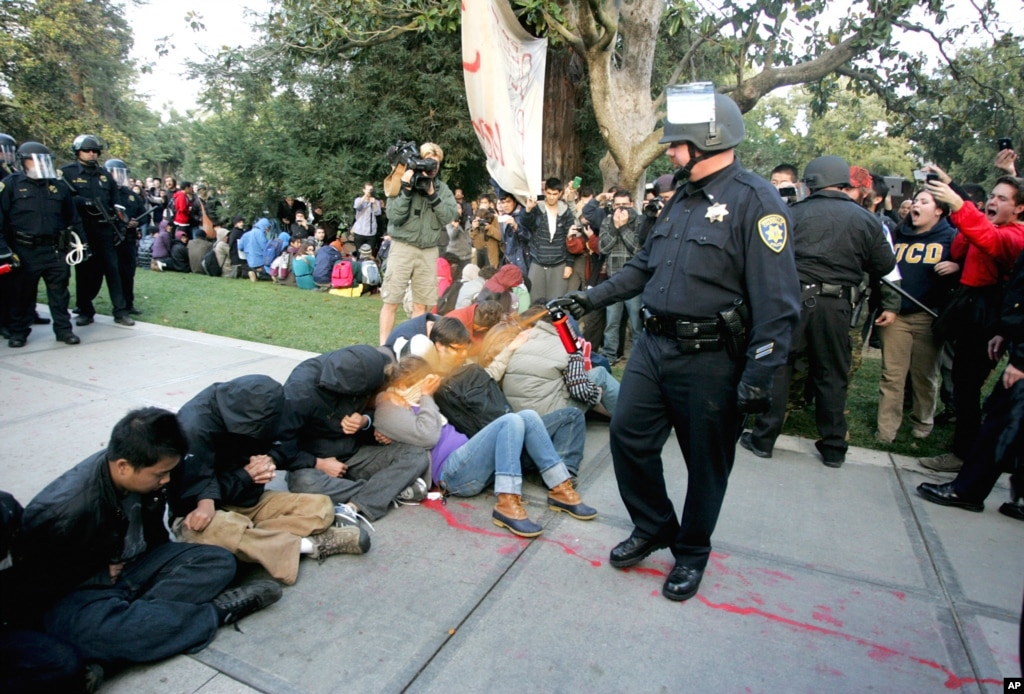
\includegraphics[width=4.25in]{graphics/pike.jpg}

In it, Lt. John Pike of the University of California Davis police force, is using pepper spray on a number of peacefully assembled and protesting students.
This incident sparked outrage across the country, and quickly, use of this picture of Pike became a symbol of government's oppressive response to the protests.
It, along with some of the political commentary about it, became so widely-known that it rose to the level of an ``internet meme.''\footnote{See: http://knowyourmeme.com/memes/casually-pepper-spray-everything-cop}

All negative government response in the following several months would be characterized by this photo, particularly police actions (unsurprisingly).
Yet, Lt. Pike's actions were not heavily punished, and the scandal has fallen out of the public consciousness.\footnote{In fact, recently, Lt. Pike was awarded around \oldstylenums{\$38,000} in a settlement due to psychological trauma resulting from the incident---more than each of the students was awarded in the legal battle immediately following the incident (see: http://www.huffingtonpost.com/2013/10/23/pepper-spray-cop-settlement\_n\_4152147.html).}
As a result of the failure of memory, Lt. Pike's interaction with Occupy had very little lasting affect.
Those which had more staying power were much simpler messages.

\subsection{The ``\oldstylenums{99} Percent''}
Arguably one of the clearest pieces of evidence that Occupy had a lasting impact on the political climate in the United States is the prevalence of particular phrases and concepts that, before Occupy, had been non-existent.
Some phrases had fairly minimal change, where others noticed massive increases.
The following charts show the highest percent relative prevalence\footnote{This is a relative measure of prevalence comparing the number of mentions of any given sample to the maximum number of mentions.} of the term's usage per year from \oldstylenums{2004--2013}.\footnote{Though this is a valid representation of the data, it is somewhat misleading. In reality, the relative prevalence across \oldstylenums{2004--2010} was significantly lower. A better representation of this data would be to use the average (rather than the highest) per year.}
The first phrase I investigated was ``wealth inequality.''

%Also see http://fair.org/extra-online-articles/bored-with-occupy8212and-inequality/, as referenced by Milkman\footcite[38]{milkman13}

\begin{tikzpicture}
   \begin{axis}[xlabel=Year, 
                ylabel=Percent, 
                title={Relative Prevalence of ``wealth inequality'' across \oldstylenums{2004--2013}},
                xticklabel style={/pgf/number format/1000 sep=}]
      \addplot table{
         X    Y
         2004 0
         2005 15
         2006 11
         2007 11
         2008 11
         2009 8
         2010 13
         2011 28
         2012 15
         2013 100
      };
   \end{axis}
\end{tikzpicture}

This chart shows fairly constant prevalence across \oldstylenums{2005 through 2010 around 15 percent}.
Then, in \oldstylenums{2011}, the year Occupy burst into public view, relative prevalence nearly doubled to a peak of \oldstylenums{28} percent.
Following a short decrease during \oldstylenums{2012, 2013} has seen the highest prevalence in history.
In simple terms, where ``wealth inequality'' had been almost entirely unmentioned until \oldstylenums{2005}, and did not see wide mention until \oldstylenums{2011} after Occupy's inception, and following the occupations, it was mentioned more last year than in any year previous.

Striking as this pattern is, ``wealth inequality'' had, at least, been discussed before Occupy got off the ground.
A better example of the shift would be tracking a phrase that had almost no exposure before the occupations.
The most obvious example of one such phrase is the now common-place term for the public---the ``\oldstylenums{99} percent.''

\begin{tikzpicture}
   \begin{axis}[xlabel=Year, 
                ylabel=Percent, 
                title={Relative Prevalence of ``\oldstylenums{99} percent'' across \oldstylenums{2006--2013}},
                xticklabel style={/pgf/number format/1000 sep=}]
      \addplot table{
         X    Y
         2004 0
         2005 0
         2006 0
         2007 0
         2008 0
         2009 0
         2010 0
         2011 100
         2012 18
         2013 11
      };
   \end{axis}
\end{tikzpicture}

The ``\oldstylenums{99} percent'' had, relatively, seen no mention whatsoever.
During Occupy, as its message largely used this phrase, its peak was reached.
However, even following the evictions and Occupy falling out of public view, it has remained stable around \oldstylenums{10} percent of its peak.\footnote{Statistically speaking, this is an infinite percent increase, but that is not a terribly helpful way of describing the pattern. I need to figure out a way of conveying, in words, how significant this difference is.}

\section{The World}

\newpage
\printbibliography
\end{document}
